\section{Exact Clairvoyant Algorithm}
\label{sec:exactalgo}

% In a real world crowdsourcing environment, the server has no information with regard to tasks (workers) becoming available in the future. The server becomes aware of a task (worker) and all its subsequent information only when the task (worker) becomes available. Due to this lack of knowledge, at each time, the server might make an assignment that will prove not to be towards an optimal solution once more information becomes available in the future. 
In order to solve the TASC problem, the server requires a global knowledge of all the current and incoming spatial tasks and workers. In such case, the server can assign tasks to workers such that the value of the matching is maximized. However, the server does not have such global knowledge. The server will become aware of a task (worker) and all its corresponding information once the task (worker) becomes available. Due to this lack of future knowledge, finding a globally optimal solution is not feasible.\\

In this section, we assume there exists a clairvoyant server which has a global knowledge of tasks and workers. The result of this algorithm can later serve as an upper bound to evaluate how well the server assigns tasks to workers. We propose a two step algorithm which finds the optimal solution to TASC problem. In the first step we find all potential subsets of tasks that a single worker is able to complete. Having the output of step 1, in the next step we find a matching with maximum value. In the following sections, we describe different steps of the algorithm and later discuss the complexity of the algorithm. At the end, we show how to adopt the algorithm to address a more general spatial crowdsourcing framework. This adoption does not deteriorate the performance of the algorithm, and in most cases will even improve it.

\subsection{Discovering Potential Task Subsets}
\label{subsec:FindPTS}
In the first step of the algorithm we focus on finding all task subsets that a worker \emph{w} will be able to complete. We can define a Potential Task Subset as:

\begin{definition} [Potential Task Subset]
\label{def:PTS}
We call $PTS \subset T$ a potential task subset for worker w iff there exists a route that starts from w.l and for every $t \in PTS$ the path visits t.l at time $\delta$ such that $t.r \leq \delta < t.d$. Also the path should not start earlier than w.s and end before w.e. We define the value of PTS as:
\begin{equation*}
Value(PTS) = \sum_{t \in PTS} t.v
\end{equation*}
\end{definition}

For each worker \emph{w}, we define \emph{w.PTS} as the union of all such potential task subsets.\\

In order to find all PTSs for a single worker, a straightforward method is to go through all subsets of \emph{T} and check whether it's a PTS for the worker or not. It's trivial to see that such approach will require $O(n!)$ permutations which makes it computationally expensive. Therefore we will adopt a branch and bound algorithm similar to the one introduced in \cite{deng13}. We use the following propositions for pruning purposes in our branch and bound algorithm.

\begin{proposition}
\label{prop:overlap}
For every $t \in T$ and $w \in W$ if $\left(t.r, t.d \right] \cap \left( w.s, w.e \right] = \emptyset$ then for every $PTS \in w.PTS$ we have $t \not\in PTS$.
\end{proposition}

\begin{proposition}
\label{prop:size}
For any $w \in W$ for every $PTS \in w.PTS$ we have $\left\vert{PTS}\right\vert \leq w.max$.
\end{proposition}

\begin{proposition}
\label{prop:subset}
For every $w \in W$ if $PTS \in w.PTS$ for every $pts \subset PTS$ we will have $pts \in w.pts$
\end{proposition}
We model the entire solution space as a tree (\cref{fig:PTS_tree}) and use a depth-first approach to search the solution space. By \cref{prop:size} we know that we only have to extend the tree up to depth $w.max$ levels for worker $w$. Each node of the tree corresponds to a subset of \emph{T}. Therefore, for any node \emph{n} of the tree, if the corresponding subset of \emph{n} is not in \emph{w.PTS}, according to \cref{prop:subset}, then we can prune the entire sub-tree rooted at \emph{n}.

\begin{figure}[t]
	\centering
	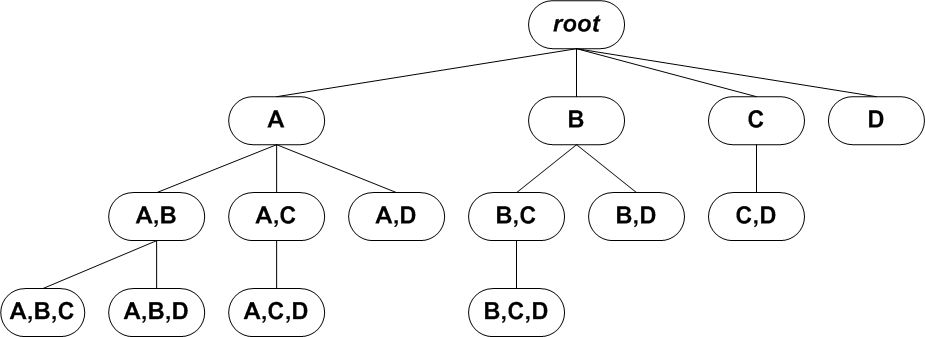
\includegraphics[width = 0.85\columnwidth]{figures/PTS_tree.png}
			\vspace{-0.2cm}
	\caption{PTS search space for $\left\vert T \right\vert = 4$ and $w.max=3$}
	\label{fig:PTS_tree}
			\vspace{-0.2cm}
\end{figure}

\begin{algorithm}[h]
\caption{FindPTSs($T, W$)}
\label{algo:FindPTS}
\begin{algorithmic}[1]
\REQUIRE \emph{T} is the set of all tasks and \emph{W} is the set of all workers
\ENSURE \emph{PTSs[]} is the list containing all potential task subsets for different workers.
\FOR{$w$ in $W$}
	\STATE $PTSs[w] = $ SearchBranch($\emptyset, T, w$)
\ENDFOR
\RETURN $PTSs$
\end{algorithmic}
\end{algorithm}

\begin{algorithm}[t]
\caption{SearchBranch($pts, T, w$)}
\label{algo:SearchBranch}
\begin{algorithmic}[1]
\REQUIRE \emph{pts} is the current subset, \emph{T} is the list of remaining tasks and \emph{w} is the worker
\ENSURE \emph{PTSs} is the set of all potential task subsets for \emph{w}
\STATE $PTSs = \emptyset$
\STATE $T_{copy} = T$
\FOR{$t$ in $T_{copy}$}
	\STATE $T = T \setminus t$
	\IF{$t$ doesn't temporally overlap with $w$}
		\STATE continue
	\ENDIF
	\STATE $s = t \cup pts$
	\IF{IsPotentialSubset($s, w$)}
		\STATE $PTSs = PTSs \cup t$
		\IF{$\left\vert{s}\right\vert < w.max$ and $T \neq \emptyset$}
			\STATE $S =$ Search\_Branch($s, T, w$)
			\STATE $PTSs = PTSs \cup S$
		\ENDIF
	\ENDIF
\ENDFOR
\RETURN $PTSs$
\end{algorithmic}
\end{algorithm}

\begin{algorithm}[t]
\caption{IsPotentialSubset($s, w$)}
\label{algo:IsPTS}
\begin{algorithmic}[1]
\REQUIRE $s$ is the input set
\ENSURE $true$ if $s$ is a PTS for $w$ and $false$ otherwise
\STATE $loc = w.l$
\STATE $time = w.s$
\FOR{$P$ in PermutationsOf($s$)}
	\STATE $possible = true$
	\FOR{$i=1$ to $\left\vert{P}\right\vert$}
		\STATE $nextTime = $max($P[i].r, time +$ dist($w.l, P[i].l$)
		\IF{$nextTime < P[i].d$ and $nextTime < w.e$}
			\STATE $loc = P[i].l$
			\STATE $time = nextTime$
		\ELSE
			\STATE $possible = false$
			\STATE break
		\ENDIF
	\ENDFOR
	\IF{$!possible$}
		\STATE continue
	\ELSE
		\RETURN $true$
	\ENDIF
\ENDFOR
\RETURN $false$
\end{algorithmic}
\end{algorithm}

\cref{algo:SearchBranch} finds all the PTSs under a specific branch of the search space. The current subset ($pts$) is expanded with a new task ($t$) if $w$ temporally overlaps with $t$ (lines 4-8). If the new subset $s$ is a PTS itself we continue the search for more PTSs in the sub-tree rooted at $s$ (lines  9-15). \cref{algo:IsPTS} checks if a subset $s$ can be a PTS for $w$. According to \cref{def:PTS}, the desired path should start from the current location of $w$ and no sooner than the time the worker becomes available (lines  1-2). We consider all permutations of $s$ and check if a permutation satisfies all the temporal constraints of \cref{def:PTS} (lines 5-14). The subset $s$ will be a PTS only if a permutation is found to satisfy all constraints. Finally in \cref{algo:FindPTS} for each worker we search for PTSs starting the search at the root of the tree.
			
\subsection{Finding the Maximal Matching}
\label{subsec:FindMM}
Having found all PTSs for each worker in step 1, the next step of the algorithm focuses on finding the matching with the maximum value. For this purpose, we construct a graph such that each PTS from step 1 is a vertex in the graph. We call this graph the \emph{PTS-Graph}. Then we show that the \emph{maximum weighted clique} in the PTS-Graph corresponds to the matching with the maximum value.

The PTS-Graph is a multi-layered graph such that for each worker we add a layer to the graph. Withing each layer $l$, for each PTS inside $w_l.PTS$ we add a node to layer $l$. The weight of this node is equal to the value of the corresponding PTS. We use an arbitrary ordering to name the nodes within each layer of the PTS-Graph. Assuming layer $l$ contains $m$ nodes, we name them $n_{l1}$ through $n_{lm}$. Also, we define the set of edges of the PTS-Graph as:
\begin{equation}
E = \left\{ \left\langle n_{ai}, n_{bj} \right\rangle \middle | a \neq b \land \left(PTS_{ai} \cap PTS_{bj} = \emptyset \right) \right\}
\end{equation}
where $PTS_lm$ refers to the corresponding PTS of node $n_{lm}$. In other words, there will be an edge between two nodes in different layers if the corresponding PTSs of the two nodes don't contain a similar task.

Given the PTS-Graph $G(V, E)$, we associate an assignment of tasks to workers with a set of vertices $N \subset V$ as follows: if $n_{lm} \in N$, then every task $t \in PTS_{lm}$ is assigned to $w_l$.

\begin{definition} [Clique]
\label{def:clique}
For undirected graph G=(V,E), a \emph{Clique} in G is a subset $S \subset V$ of vertices, such that $\{x,y\} \in E$ for all distinct $x,y \in S$.
\end{definition}

A clique is said to be \emph{maximal} if its vertices are not a subset of the vertices of a larger clique, and \emph{maximum} if there are no larger cliques in the graph.

\begin{definition} [Maximum Weight Clique]
\label{def:maxClique}
For undirected graph G=(V,E) where each $v \in V$ is assigned a value $w(v)$, the \emph{Maximum Weight Clique} is the clique for which the sum over the weight of all vertices in the clique, is larger than any other clique in the graph.
\end{definition}

It's worth noting that a maximum weight clique is not necessarily a maximum clique but it definitely is a maximal clique.

\begin{theorem}
\label{th:maxClique}
If C* is a maximum weighted clique in the PTS-Graph, then the assignment of tasks to workers corresponding to C*, M*, will be a maximum value matching for the TASC problem.
\end{theorem}

\begin{proof}
Based on the way we generated the PTS graph, no two vertices in C* can contain the same task in their corresponding PTS. Therefore, any task t will be assigned to at most one worker. Next we need to show no other matching M can have a larger value than M*. If such matching M existed, then the clique C corresponding to M, will have a larger weight than C* which conflicts the fact that C* is the maximum weighted clique.
\end{proof}

There exists a vast body of literature on solving the maximum weight clique problem \cite{Kovalyov07}. Here we briefly explain one of these algorithms and refer the interested readers to \cite{Ostergard01}.\\

In \cref{algo:MWC} we start with an arbitrary node ordering. \cite{Ostergard01} suggests a node ordering where $v_1$ is the node with the largest total sum of the weights of its adjacent vertices and so on. \cref{algo:MWC} computes a value $C(k), 1 \leq k \leq n$ which tells the largest weight of a clique, only considering nodes $\left\{v_k, v_{k+1}, ..., v_n\right\}$. If $w(i)$ denotes the weight of $v_i$, then we will have $C(n) = w(i)$ and other values for $C()$ are computed in a backtrack search. For $1 \leq k \leq n-1, C(k) > C(k+1)$ only when a corresponding clique exists and contains $v_k$. If such clique does not exist then $C(k) = C(k+1)$. In order to find such $C(k)$ clique, a branch and bound approach is used to search all possible cliques. Details of the branch and bound algorithm can be found in \cite{Ostergard01}.

\begin{algorithm}
\caption{MaximumWeightClique($V, E$)}
\label{algo:MWC}
\begin{algorithmic}[1]
\REQUIRE $V$ is an ordering of the nodes and $E$ is the set of edges in the graph
\ENSURE $C$ a subset of $V$ as the maximum weighted clique
\STATE $C = \left\{ v_n \right\}$
\STATE $max = w(n)$
\FOR{$k: n-1$ down to $1$}
	\STATE $\left\langle C_k, w \right\rangle =$ FindMaxClique($V, E, v_k$)
	\IF{$w > max$}
		\STATE $C = C_k$
		\STATE $max = w$
	\ENDIF
\ENDFOR
\RETURN $C$
\end{algorithmic}
\end{algorithm}

\subsection{Complexity Analysis}
\label{subsec:exactcomplexity}

Here we analyze the time complexity of our proposed exact algorithm. For simplicity we assume $\left\vert T \right\vert = n$, $\left\vert W \right\vert = m$ and $\left\vert w.max \right\vert = p$. We start with \cref{algo:IsPTS}. The size of set $s$ is at most equal to $p$, hence the number of permutations of $s$ is $O(p^p)$. Also the for loop in line 5 will run at most $p$ times which will make the overall complexity of \cref{algo:IsPTS} $O(p^{p+1})$. For \cref{algo:SearchBranch} we can assume that we are running the IsPotentialPTS() method for each node of the search space tree(\cref{fig:PTS_tree}) once. At level $i$ of the search space tree we will have at most $C(n,i)$. Also for each node in level $i$ the size of the task subsets will be $i$. Hence, the IsPotentialSubset() method will run in $O(i^{i+1})$. Therefore the amortized time complexity of \cref{algo:SearchBranch} will be:

\begin{equation*}
\mathlarger{\mathlarger{\sum}}_{i = 1}^{p} \dbinom{n}{i} O(i^{i+1}) = O(n^{n-p}p^{p+1})
\end{equation*}

Since we run the SearchBranch method for each worker once in, we can conclude the the time complexity of \ref{algo:FindPTS} is $O(mn^{n-p}p^{p+1})$.\\

In \cref{algo:MWC} we implement the FindMaxClique() method, we use a branch and bound algorithm described in \cite{Ostergard01}. The time complexity of this algorithm will be $O(n^n)$ for a graph of size $n$. Therefore, for a graph of size $n$, the overall time complexity of \cref{algo:MWC} will be $O(n^{n+1})$.

\begin{theorem}
The TASC problem is NP-Complete.
\end{theorem}

\begin{proof}
By reducing the \emph{TASC} problem to a known NP-Complete problem we show the NP-Completeness of \emph{TASC}. In this section we showed how we can reduce the \emph{TASC} problem to solving a \emph{Maximum Weighted Clique (MWC)} problem. The \emph{Clique Decision} problem itself is one of Richard Karp's original 21 problems shown to be NP-Complete \cite{Karp72}.
\end{proof}

We end the section with a discussion on how generalizing the spatial crowdsourcing framework can affect the algorithm introduced in this section. In \cite{Kazemi13} it's assumed that each task requires a certain level of \emph{confidence} and only workers with a \emph{trust} level higher than than will be able to perform the task. It's also seen that in some spatial crowdsouring frameworks, workers define a spatial range and only perform task within this range. Constraints like this will only remove a subset of tasks from the list of tasks a certain worker is able to execute. As a result, the search space of \cref{algo:FindPTS} will get reduced and we end up with few number of PTSs per worker. This in turn will reduce the size of the PTS-Graph in \cref{subsec:FindMM}.